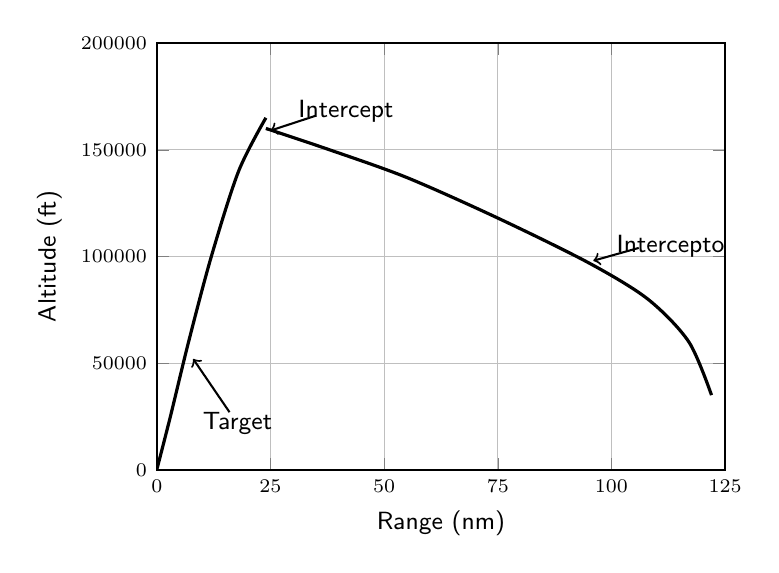
\begin{tikzpicture}
  \begin{axis}[
    width=8.8cm,height=7.0cm,
    xmin=0,xmax=125,ymin=0,ymax=200000,
    xtick={0,25,50,75,100,125},
    ytick={0,50000,100000,150000,200000},
    grid=major,
    axis line style={line width=0.8pt},
    tick label style={font=\scriptsize},
    label style={font=\sffamily\small},
    xlabel={Range (nm)},
    ylabel={Altitude (ft)},
    scaled y ticks=false,
    yticklabel style={/pgf/number format/fixed,/pgf/number format/1000 sep={}},
  ]
    \addplot[line width=1.15pt,smooth] coordinates {
      (0,0) (3,25000) (7,60000) (12,100000) (18,140000) (24,165000)
    };
    \addplot[line width=1.15pt,smooth] coordinates {
      (24,160000) (38,150000) (55,137000) (75,118000) (95,97000)
      (108,80000) (117,60000) (122,35000)
    };
    \node[font=\sffamily\small,anchor=west] at (axis cs:29,168000) {Intercept};
    \draw[->,line width=0.75pt] (axis cs:35,166000)--(axis cs:25,159000);
    \node[font=\sffamily\small,anchor=west] at (axis cs:99,105000) {Interceptor};
    \draw[->,line width=0.75pt] (axis cs:106,104000)--(axis cs:96,98000);
    \node[font=\sffamily\small,anchor=west] at (axis cs:8,22000) {Target};
    \draw[->,line width=0.75pt] (axis cs:16,27000)--(axis cs:8,52000);
  \end{axis}
\end{tikzpicture}
